%\section*{Постановка задачи}
%Необходимо сделать нормальный шаблон для отчётов в Политехе. Структура отчётов может быть разной, зависит от требования преподавателя, поэтому файл content.tex отдельно выделен от всех других в шаблоне и не делится на подчасти.

%\newpage
%\section{Заполнение шаблона}
%\begin{itemize}
	%\item Изменить \textbf{config.tex}: имя студента, название предмета и пр. %параметры указаны именно там
	%\item Заполнить \textbf{content.tex} - файл, который будет содержать весь %текст отчёта, от вступления до заключения.
	%\item Добавить используемую литературу (если есть) в \textbf{refs.bib}. Для %удобного поиска источников можно воспользоваться Google Books. Использованные %источники можно указывать с помощью команды \textbf{\\cite\{name\_of\_ref\}}
%\end{itemize}
%Далее представлены различные примеры.

\section{Теоретическая информация}
    Было использовано методическое указание по выполнению лабораторного практикума по основам фотоники. Исследование кинетических свойств фотохромных стекол. \cite{conlan1983massive}

\section{Ход выполнения работы}

\subsection{В ходе выполнения данной лабораторной работы было получено}

\begin{itemize}
	\item Коэффициенты пропускания фотохромных стекол в процессе потемнения и обесцвечивания[См. Таблицы]
	\item Рассчитана начальная оптическая плотность для каждого образца
	\item Рассчитана степень потемнения для каждого образца
	\item Рассчитан критерий релаксации для каждого образца
	\item Были получены графики зависимости оптической плотности от времени потемнения для каждого образца
\end{itemize}


\subsection{Графики}

\begin{figure}
        \centering
        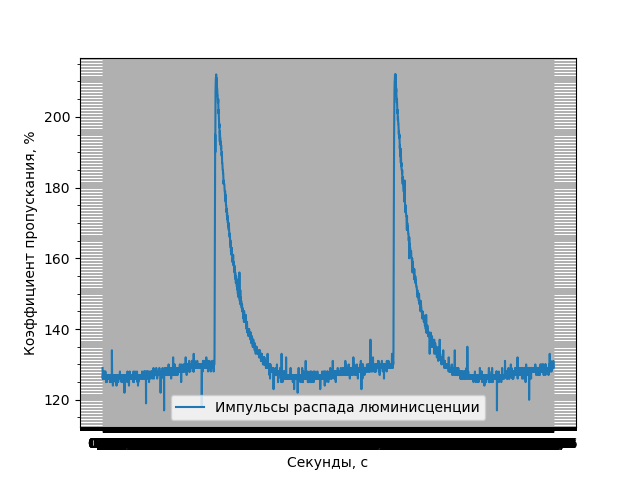
\includegraphics{figures/example}
        \caption{Какой-то график}
		\label{fig:someFigure}
\end{figure}

\section*{Заключение}
В данной работе я измерил интегральную оптическую плотность фотохромного стекла, рассчитал добавочную оптическую плотность и критерий релаксации.
Среди образцов 1-7:
\begin{itemize}
	\item Образец №2 обладает наибольшей степенью потемнения (потемнение наиболее значительно, в сравнении с остальными образцами)
	\item Образец №5 наивысшим критерием релаксации (наиболее быстрое обесцвечивание)
	\item Образец №2 обладает наивысшим показателем оптической плотности (наибольшая степень потемнения)
\end{itemize}
